\phantomsection\addcontentsline{toc}{section}{\numberline {}CHƯƠNG 4. THIẾT KẾ IP SỐ VÀ KIỂM THỬ}
\section*{CHƯƠNG 4. THIẾT KẾ IP SỐ VÀ KIỂM THỬ}
\setcounter{section}{4}
\setcounter{figure}{0}
\setcounter{table}{0}
Trong chương này, mô hình hệ thống chuyển đổi PDM sang PCM sử dụng nhiều giai đoạn đề cập ở \hyperref[chuong3]{chương 3} được thiết kế và kiểm thử ở mức Register Transfer Logic (RTL). Ngôn ngữ mô tả phần cứng SystemVerilog được sử dụng để xây dựng thiết kế cũng như testbench. Bản thiết kế cuối cùng được mô phỏng, kiểm thử trên phần mềm Mentor Questasim.
\subsection{Thiết kế}
Với yêu cầu của hệ thống số là tối ưu diện tích và công suất. Ở thiết kế này sẽ sử dụng kỹ thuật tăng tần số làm sao để một bộ nhân hoặc bộ cộng có thể thực hiện nhiều phép toán trong 1 khoảng thời gian. Với các yêu cầu như mục \ref{spec_muc}, chúng ta tiến hành thiết kế như sau.
\subsubsection{Vấn đề về tính toán fixed-point cho các hệ số của bộ lọc}
Trong phần mềm, các phép tính toán truyền thống với số dấu phẩy động đều thực hiện
trên GPU hay CPU. Nhưng khi đưa lên phần cứng, việc triển khai dấu phẩy động cực kỳ phức tạp và tốn tài nguyên. Do đó chúng ta cần chuyển đổi các hệ số của các bộ lọc sang dấu phẩy tĩnh, nhưng phải đảm bảo là các yêu cầu đặt ra với bộ lọc trước đó phải đúng.

\begin{figure}[H]
    \centering
    \includesvg[width=17cm]{Images/Chuong4/hb1.svg}
    \caption[Đáp ứng tần số của bộ lọc Half band (1) trước và sau khi sử dụng fixed-point]{\bfseries \fontsize{12pt}{0pt}\selectfont Đáp ứng tần số của bộ lọc Half band (1) trước và sau khi sử dụng fixed-point}
    \label{hb1_d}
\end{figure}


\begin{figure}[H]
    \centering
    \includesvg[width=17cm]{Images/Chuong4/hb2.svg}
    \caption[Đáp ứng tần số của bộ lọc Half band (2) trước và sau khi sử dụng fixed-point]{\bfseries \fontsize{12pt}{0pt}\selectfont Đáp ứng tần số của bộ lọc Half band (2) trước và sau khi sử dụng fixed-point}
    \label{hb2_d}
\end{figure}
Thực hiện nhân với tất cả các hệ số của bộ lọc với $2^N$ với N chạy từ 0 đến khi nào thỏa mãn được các điều kiện đặt ra. Khi ở giá trị N = 20, chúng ta thu đáp ứng tần số của các bộ lọc lần lượt như hình \ref{hb1_d}, \ref{hb2_d}, \ref{fir_d}.
\begin{figure}[H]
    \centering
    \includesvg[width=17cm]{Images/Chuong4/fir.svg}
    \caption[Đáp ứng tần số của bộ lọc FIR trước và sau khi sử dụng fixed-point]{\bfseries \fontsize{12pt}{0pt}\selectfont Đáp ứng tần số của bộ lọc FIR trước và sau khi sử dụng fixed-point}
    \label{fir_d}
\end{figure}
Theo chúng ta quan sát, bộ lọc chỉ biến thiên lớn ở thông số suy giảm giải dừng, còn độ gợn sóng và các thông số còn lại hầu như không thay đổi. Độ suy giảm dải dừng giảm từ 0.794 dB đối với FIR, 3 và 5 dB với 2 bộ lọc còn lại, tuy nhiên độ suy giảm đó vẫn lớn hơn 89 dB (yêu cầu của hệ thống).

\textbf{Kết luận}: Chúng ta sẽ sử dụng tất cả hệ số nhân với $2^20$ để ép thành số nguyên (hệ thập phân), đồng nghĩa với việc sau mỗi bộ lọc, kết quả phải dịch phải 20 lần.
\subsubsection{Mô tả chung}
Bộ chuyển đổi PDM sang PCM nhiều giai đoạn sử dụng Decimation (dti\_pdm2pcm) chuyển đổi dữ liệu PDM 1 bit với tốc lấy mẫu cao thành dữ liệu PCM với  tốc độc lấy mẫu thấp hơn. Tần số cấp cho bộ gấp 4 lần tần số lấy mẫu của PDM, từ tần số này sẽ cấp và chia tần ra các tần số cần thiết cho dti\_pdm2pcm. Tín hiệu PCM đầu ra sẽ đi kèm theo sườn dương của tín hiệu đồng hồ PCM đầu ra với độ rộng bit do người dùng quyết định (16 - 32 bit), độ rộng càng lớn thì chất lượng âm thanh đầu ra càng cao. Sơ đồ chân của dti\_pdm2pcm được mô tả như hình \ref{top_pdm2pcm}.

\begin{figure}[H]
    \centering
    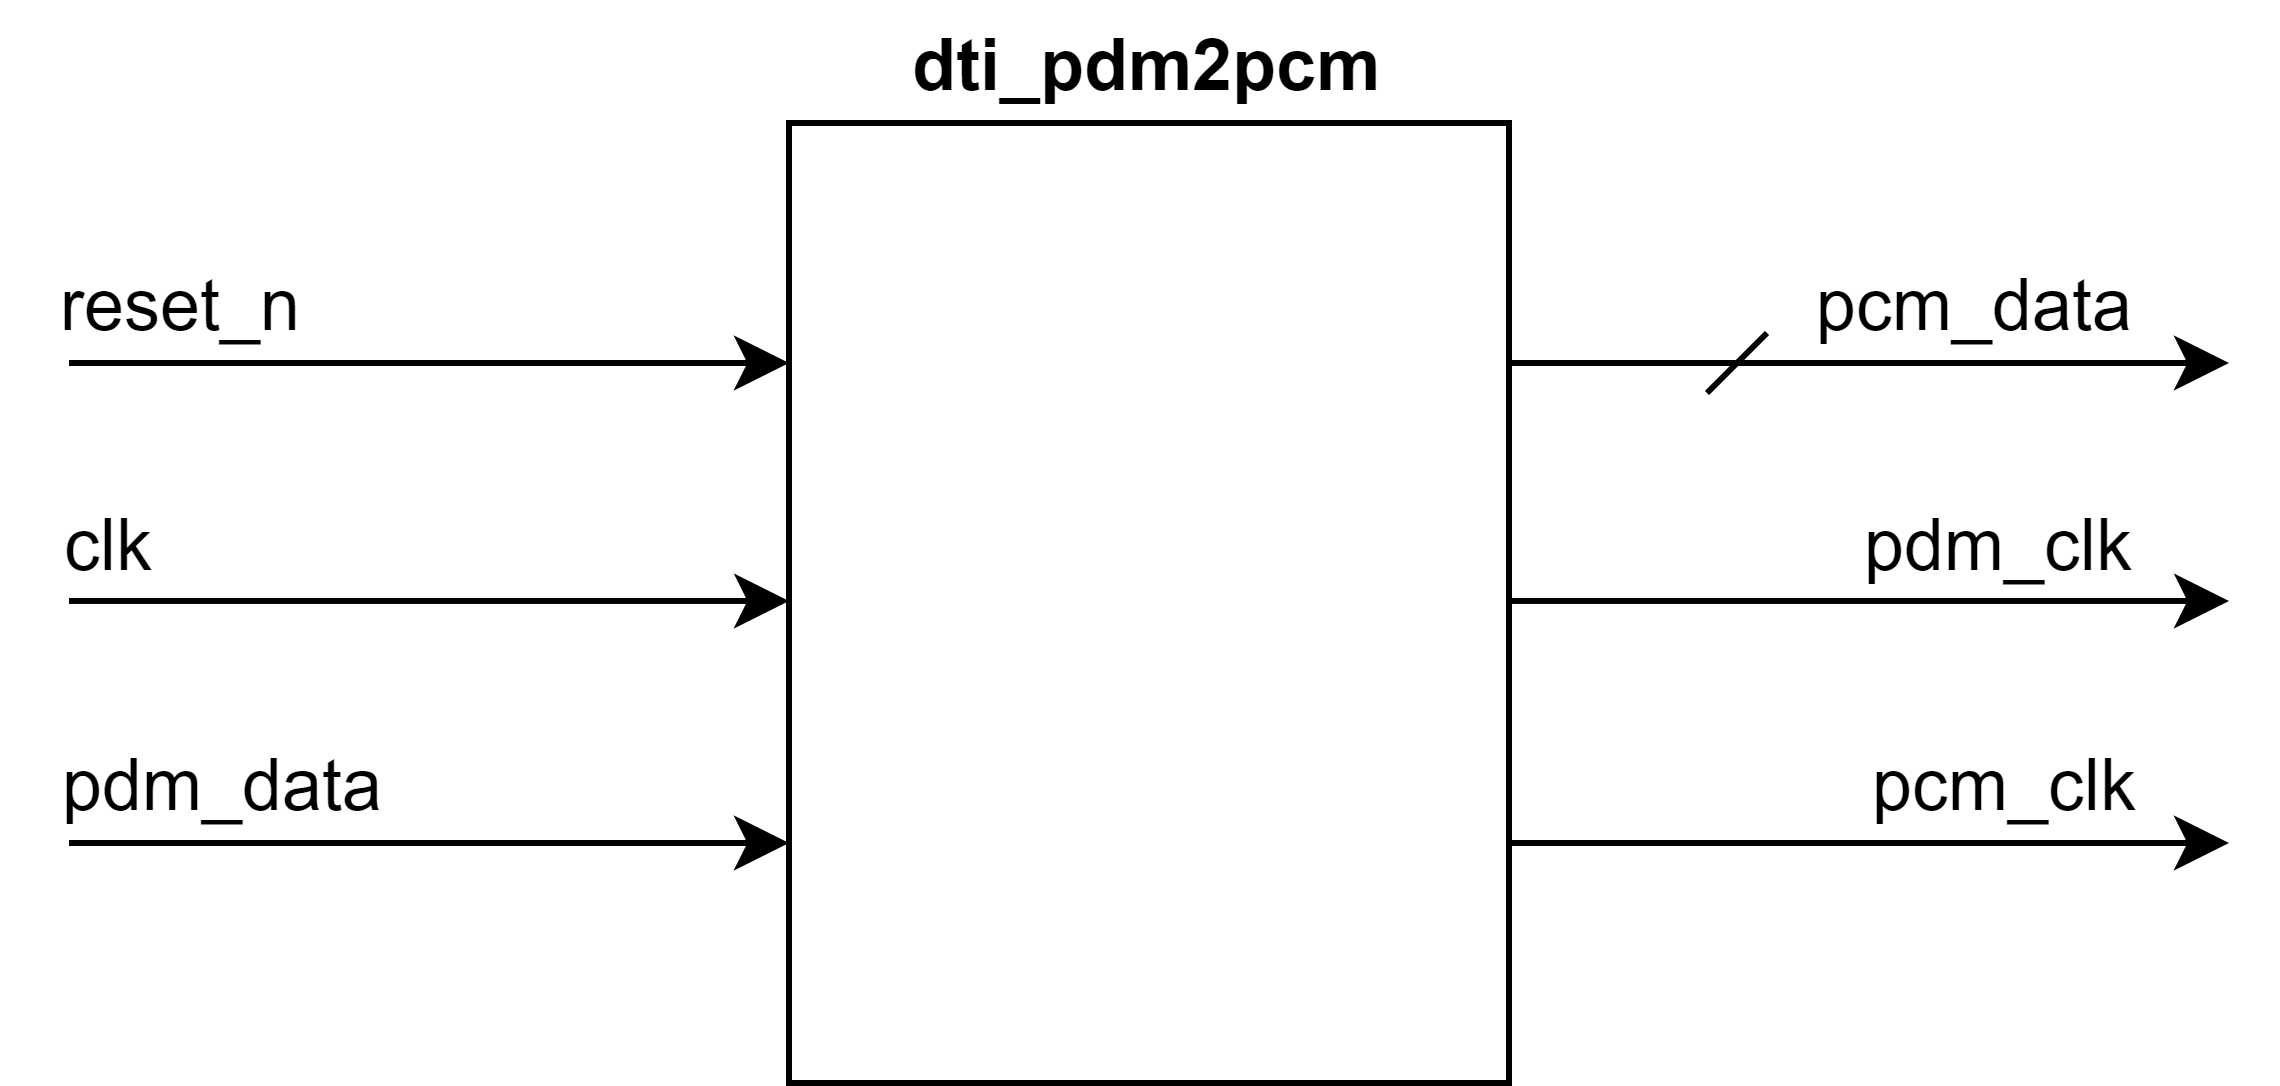
\includegraphics[width=10cm]{Images/Chuong4/top.png}
    \caption[Sơ đồ tổng quát của bộ PCM2PDM]{\bfseries \fontsize{12pt}{0pt}\selectfont Sơ đồ tổng quát của bộ PCM2PDM}
    \label{top_pdm2pcm}
\end{figure}
Các chân của bộ chuyển đổi sẽ được trình bày chi tiết ở bảng \ref{top_signal}.

Bảng \ref{hangso} mô tả các hẳng số được sử dụng trong thiết kế.

\begin{table}[H]
    \centering
    \caption[Mô tả chân vào ra của hệ thống]{\bfseries\fontsize{12pt}{0pt}\selectfont Mô tả chân vào ra của hệ thống}
\begin{tabular}{|c|c|c|l|}
\hline
\textbf{Tên chân} & \textbf{Vào/ ra} & \textbf{Độ rộng bit} & \multicolumn{1}{c|}{\textbf{Mô tả chức năng}}                                               \\ \hline
clk       & vào & 1          & Clock đồng bộ hoạt động của hệ thống \\ \hline
reset\_n          & vào              & 1                    & \begin{tabular}[c]{@{}l@{}}Chân reset không đồng bộ, tích cực mức\\ thấp\end{tabular}       \\ \hline
pdm\_data & vào & 1          & Dữ liệu từ MEMS, dạng PDM            \\ \hline
pdm\_clk  & ra  & 1          & Clock lấy mẫu của dữ liệu PDM        \\ \hline
pcm\_data & ra  & PCM\_WIDTH & Dữ liệu PCM sau khi được chuyển đổi  \\ \hline
pcm\_clk          & ra               & 1                    & \begin{tabular}[c]{@{}l@{}}Clock đi cùng dữ liệu PCM, dùng cho thiết\\ bị khác\end{tabular} \\ \hline
\end{tabular}
    \label{top_signal}
\end{table}
\begin{table}[H]
    \centering
    \caption[Hằng số thiết kế]{\bfseries\fontsize{12pt}{0pt}\selectfont Hằng số thiết kế}
\begin{tabular}{|l|c|l|}
\hline
\multicolumn{1}{|c|}{\textbf{Hằng số}} & \textbf{Giá trị} & \multicolumn{1}{c|}{\textbf{Mô tả}} \\ \hline
PCM\_WIDTH  & 24 & Độ rộng của tín hiệu PCM đầu ra \\ \hline
MULP\_WIDTH & 21 & Kích thước đầu vào của bộ nhân  \\ \hline
FIR\_SIZE   & 51 & Số lượng taps của bộ lọc FIR    \\ \hline
HB1\_SIZE   & 11 & Số lượng taps của bộ lọc HB1    \\ \hline
HB2\_SIZE   & 19 & Số lượng taps của bộ lọc HB2    \\ \hline
\end{tabular}
    \label{hangso}
\end{table}
\subsubsection{Kiến trúc}
Sơ đồ tổng quan của kiến trúc được mô tả như hình \ref{arc_top}.
\begin{figure}[H]
    \centering
    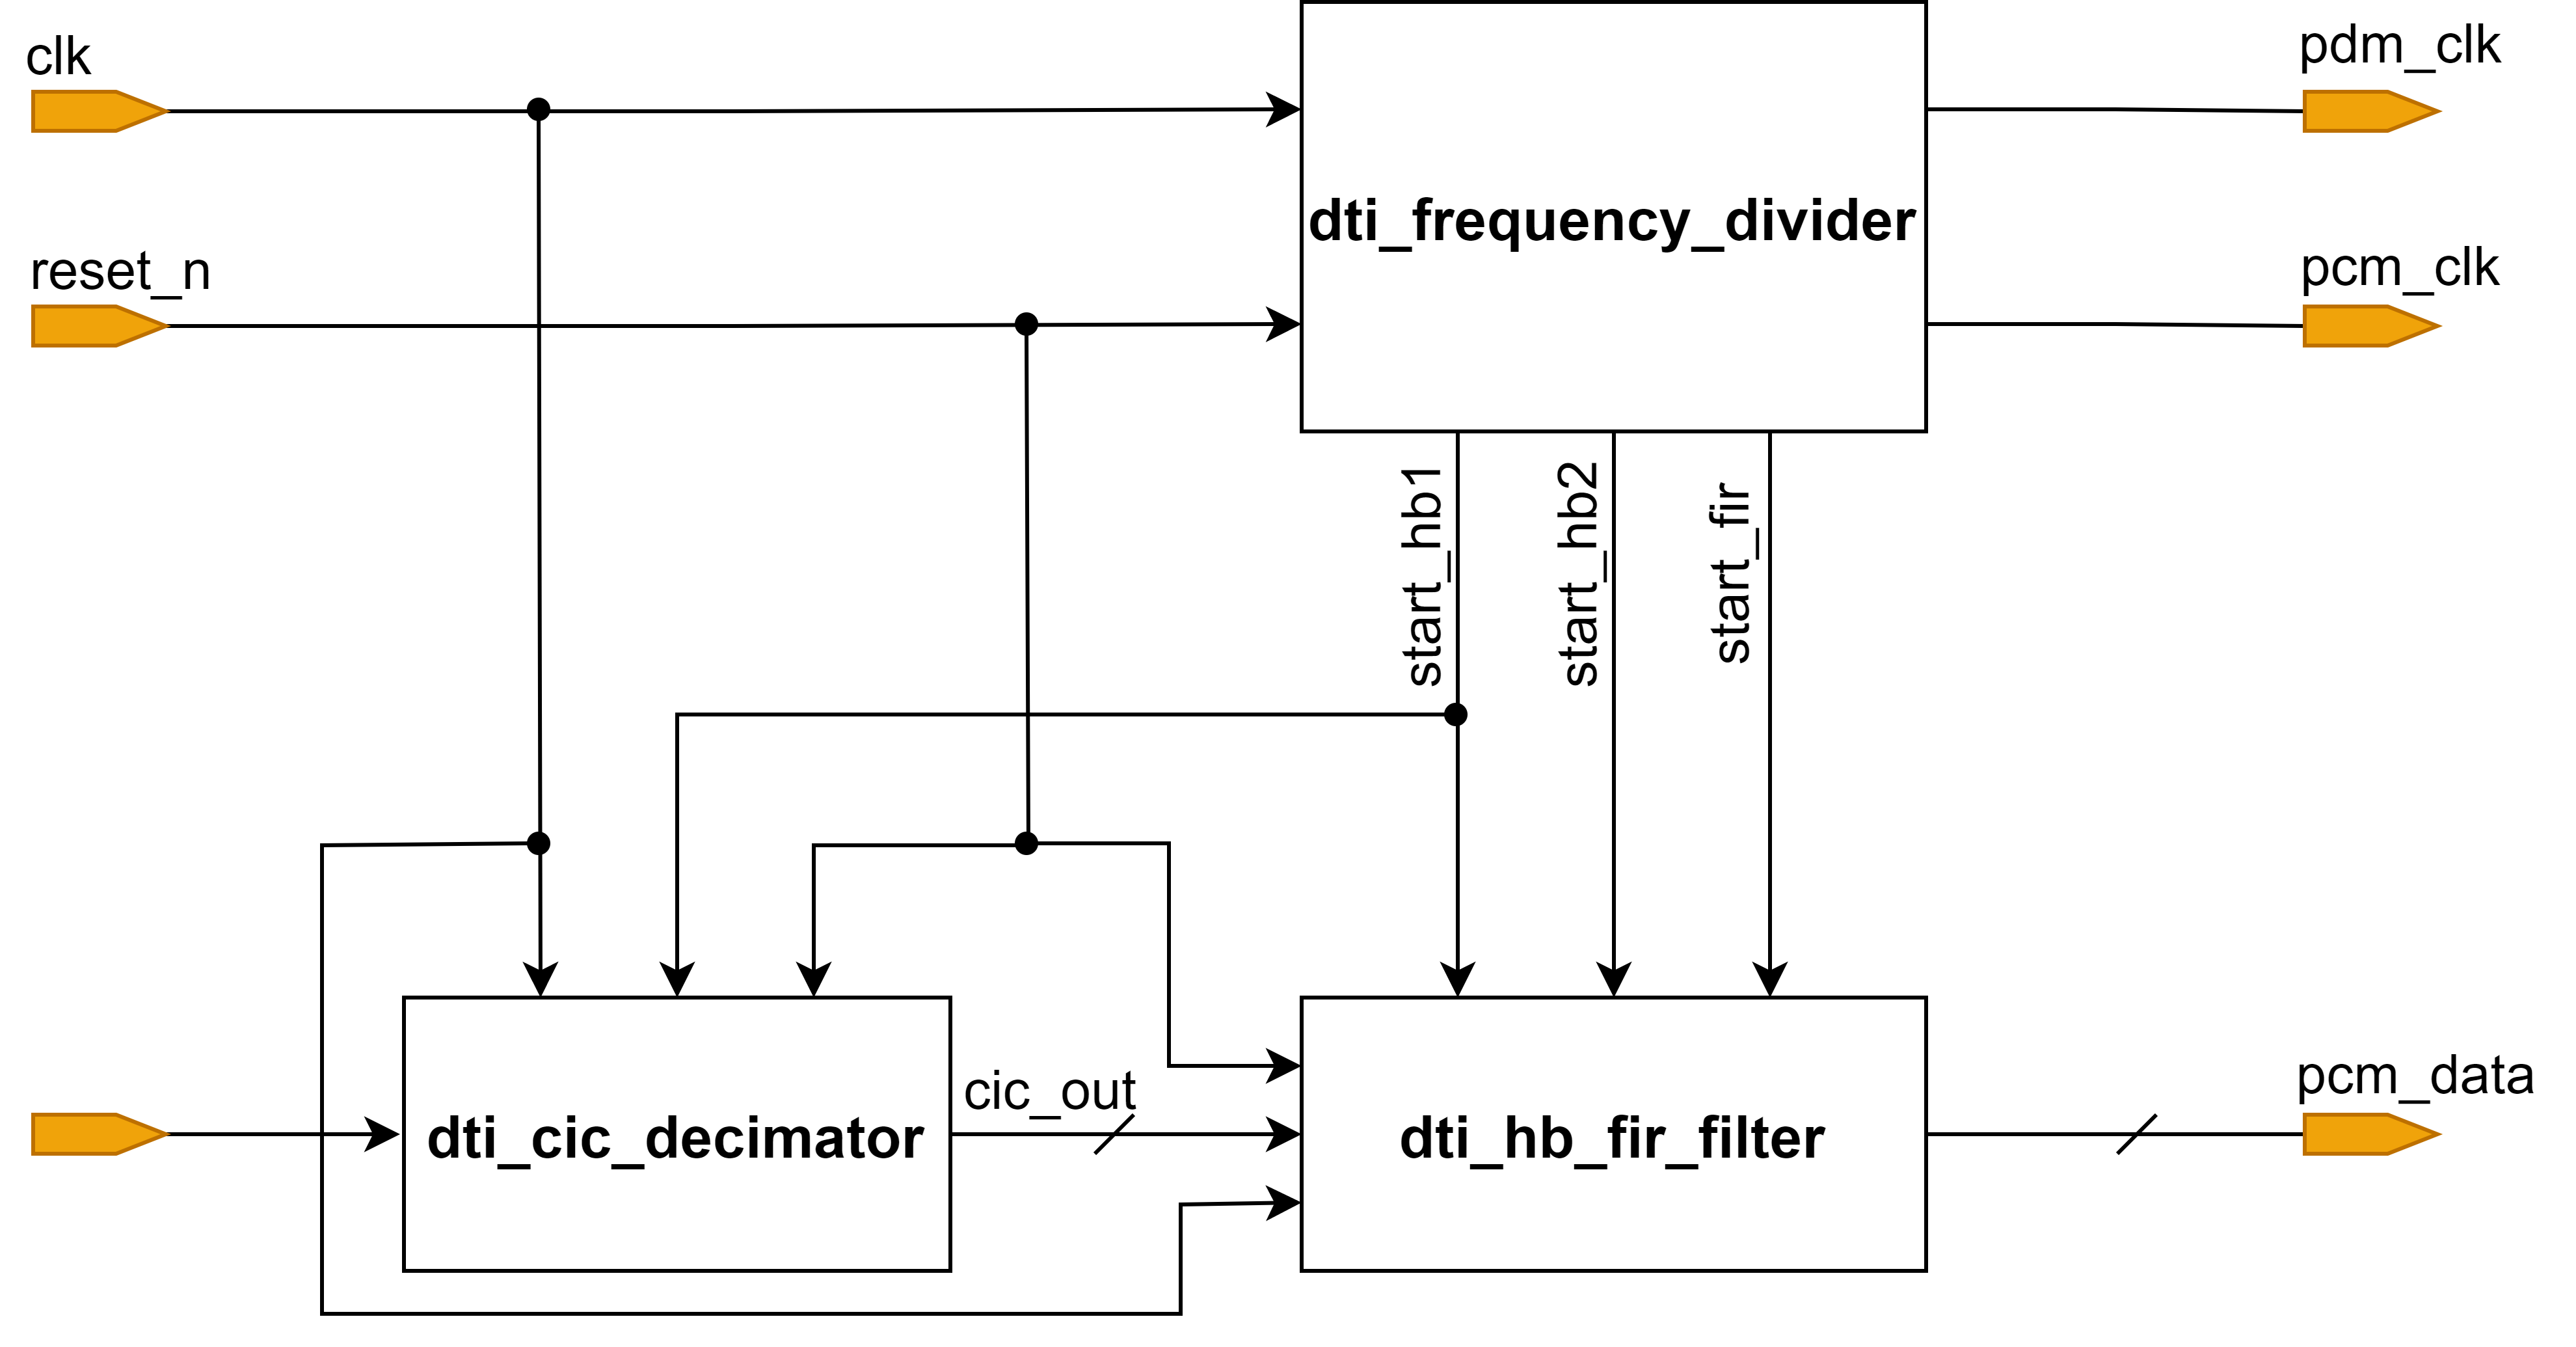
\includegraphics[width=13cm]{Images/Chuong4/arc_top.png}
    \caption[Kiến trúc của bộ PCM2PDM]{\bfseries \fontsize{12pt}{0pt}\selectfont Kiến trúc của bộ PCM2PDM}
    \label{arc_top}
\end{figure}

Chức năng của từng khối :
\begin{itemize}
    \item \textbf{dti\_frequency\_divider} đóng vai trò là bộ điều khiển, nó tạo ra tín hiệu điều khiển để khởi động hoạt động của các thành phần bên trong khối khác. Nó hoạt động như bộ chia tần.
    \item \textbf{dti\_cic\_decimator} là một bộ lọc CIC với hệ số decimation 12x và 4 tầng.
    \item \textbf{dti\_hb\_fir\_filter} là một nhóm gồm 2 bộ lọc Half Band và 1 bộ lọc FIR với tổng hệ số Decimation là 4. Vai trò của chúng là lấy mẫu xuống và bù tín hiệu.
\end{itemize}
\subsubsection{Thiết kế chi tiết từng khối}
\paragraph{dti\_frequency\_divider}
\textbf{dti\_frequency\_divider} có chức năng chia tần số từ clock đầu vào thành clock có tần số bé hơn với tỷ lệ DECIMATION là tỷ lệ chia tần. Đồng thời tạo ra tín hiệu báo hiệu quá trình đổi tần.

Sơ đồ chân vào ra của khối được mô tả ở hình \ref{frequency}.

\begin{figure}[H]
    \centering
    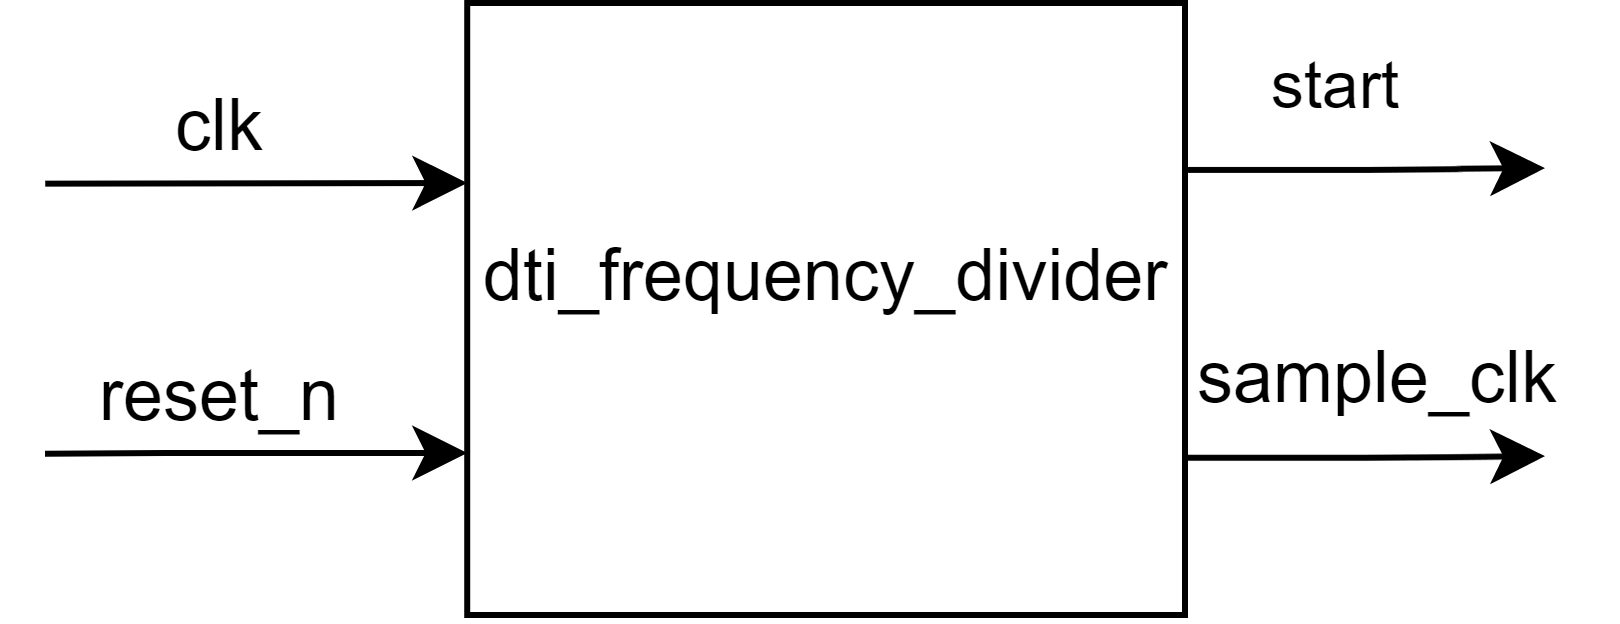
\includegraphics[width=8cm]{Images/Chuong4/frequency/frequency.png}
    \caption[Sơ đồ khối của dti\_frequency\_divider]{\bfseries \fontsize{12pt}{0pt}\selectfont Sơ đồ khối của dti\_frequency\_divider}
    \label{frequency}
\end{figure}
Bảng \ref{frequency_t} mô tả các chân vào ra của khối.
\begin{table}[H]
    \centering
    \caption[Mô tả chân vào ra của dti\_frequency\_divider]{\bfseries\fontsize{12pt}{0pt}\selectfont Mô tả chân vào ra của dti\_frequency\_divider}
    \begin{tabular}{|l|c|c|l|}
\hline
\multicolumn{1}{|c|}{\textbf{Tên chân}} &
  \textbf{Vào/ ra} &
  \textbf{Độ rộng bit} &
  \multicolumn{1}{c|}{\textbf{Mô tả chức năng}} \\ \hline
clk         & vào & 1 & Clock đồng bộ hoạt động của hệ thống \\ \hline
reset\_n &
  vào &
  1 &
  \begin{tabular}[c]{@{}l@{}}Chân reset không đồng bộ, tích cực mức\\ thấp\end{tabular} \\ \hline
start &
  ra &
  1 &
  \begin{tabular}[c]{@{}l@{}}Tín hiệu điều khiển, cho biết dữ liệu đầu \\ vào bộ lọc đã sẵn sàng\end{tabular} \\ \hline
sample\_clk & ra  & 1 & Clock đã được hạ tần                 \\ \hline
\end{tabular}
    \label{frequency_t}
\end{table}
\begin{figure}[H]
    \centering
    
\includegraphics[width=15cm]{Images/Chuong4/frequency/frequency_timing.png}
    \caption[Biểu đồ thời gian của dti\_frequency\_divider]{\bfseries \fontsize{12pt}{0pt}\selectfont Biểu đồ thời gian của dti\_frequency\_divider}
    \label{frequency_t}
\end{figure}

Kiến trúc của khối được mô tả ở hình \ref{frequency_a}, quá trình hoạt động tương ứng được biểu diễn như hình \ref{frequency_t}.

\begin{figure}[H]
    \centering
    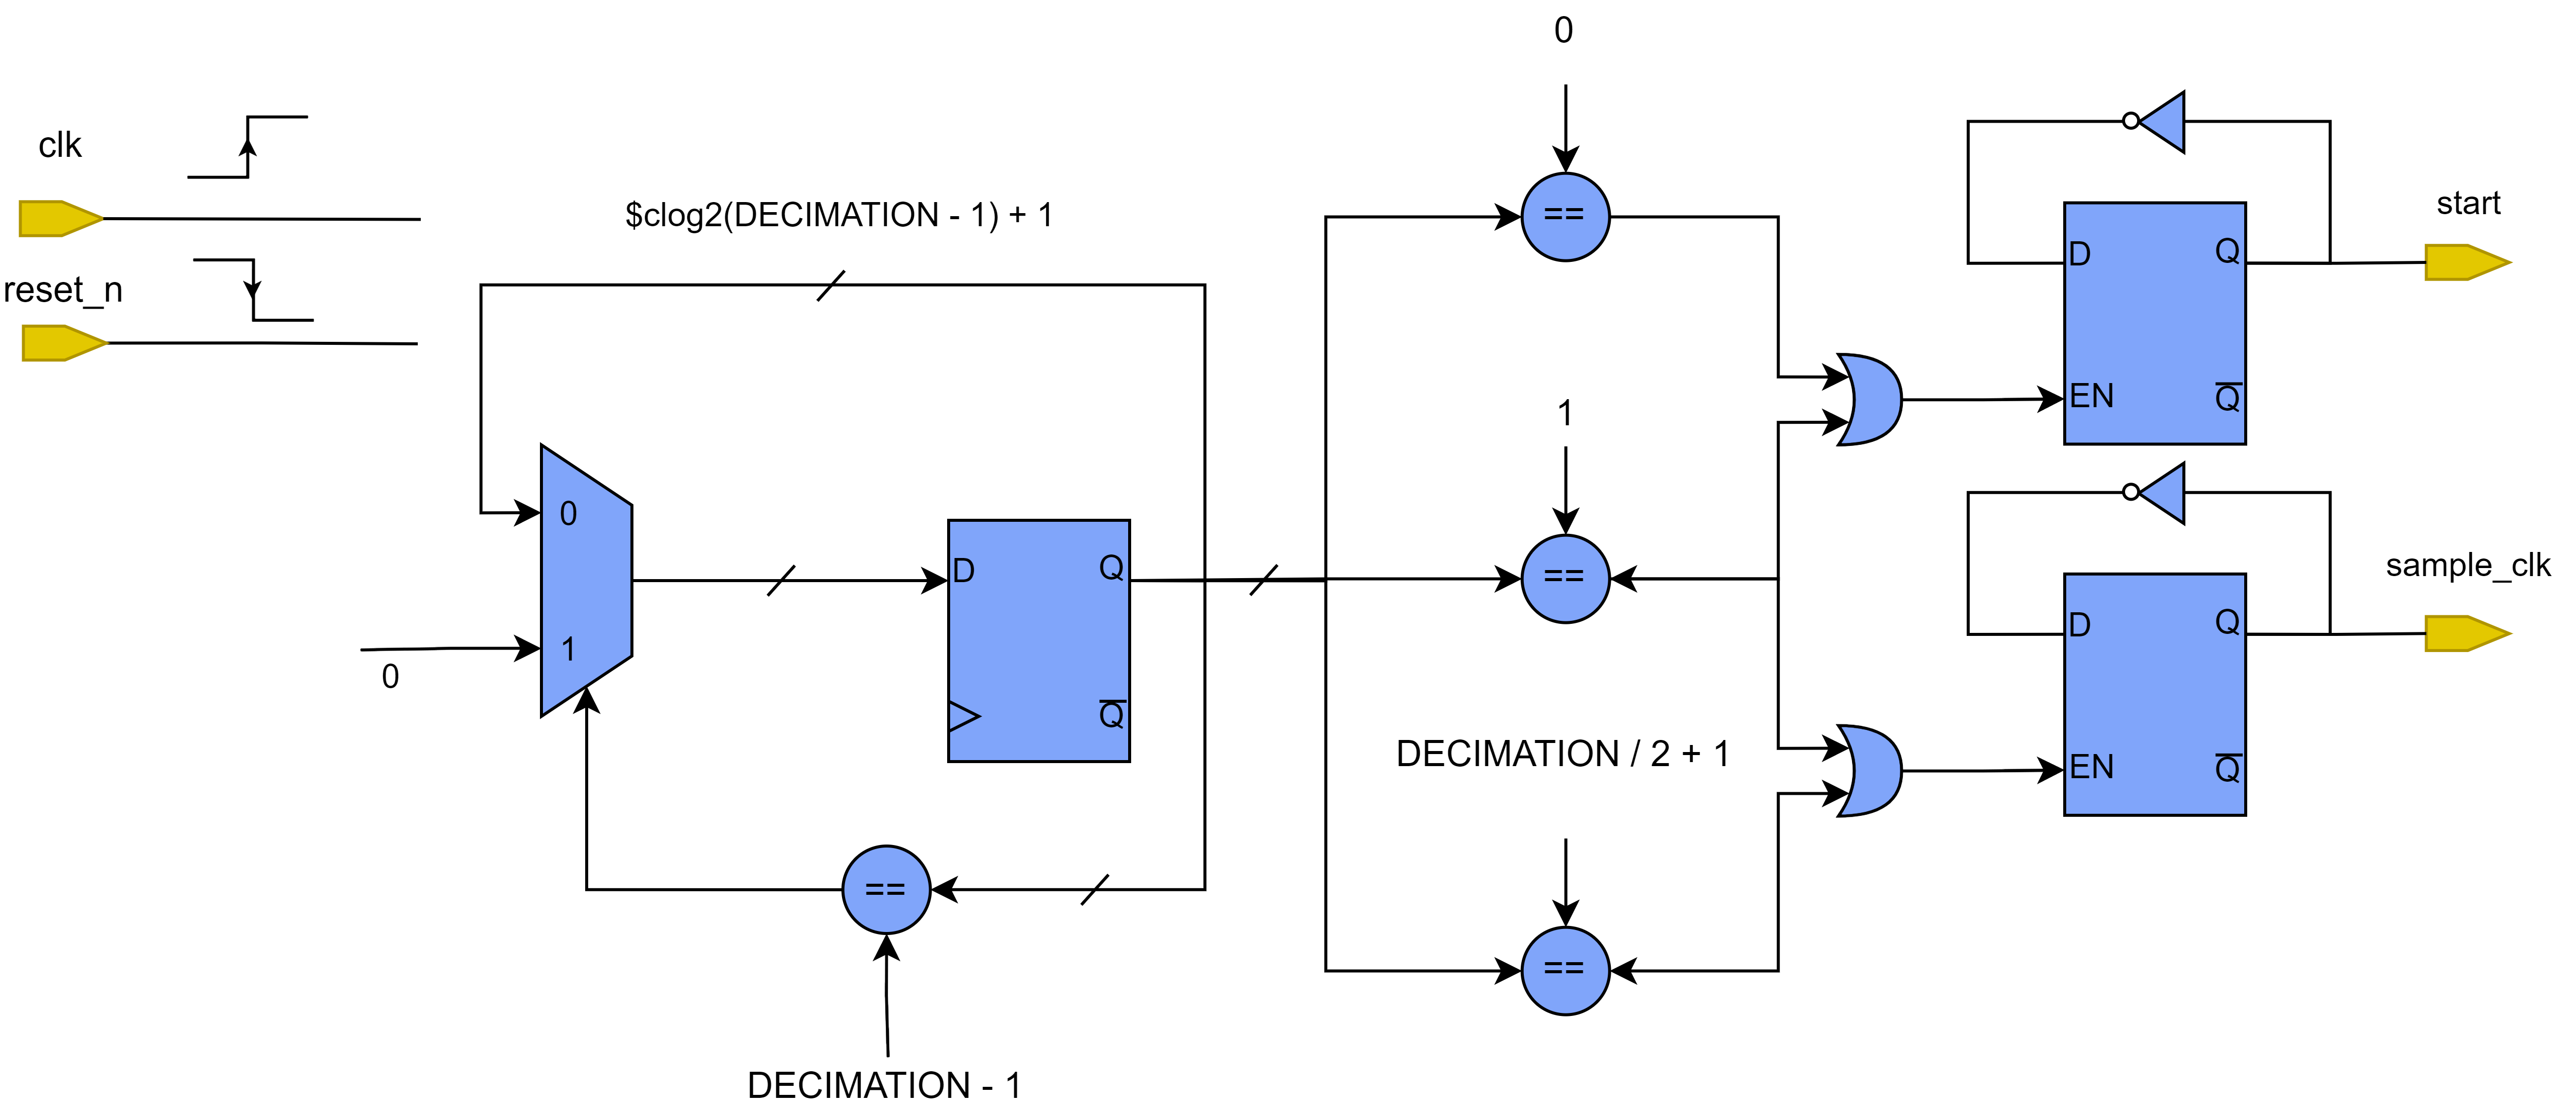
\includegraphics[width=14cm]{Images/Chuong4/frequency/frequency_arc.png}
    \caption[Kiến trúc của dti\_frequency\_divider]{\bfseries \fontsize{12pt}{0pt}\selectfont Kiến trúc của dti\_frequency\_divider}
    \label{frequency_a}
\end{figure}

\paragraph{dti\_top\_frequency\_divider}
\textbf{dti\_top\_frequency\_divider} (hình \ref{top_frequency}) chứa các \textbf{dti\_frequency\_divider} với hệ số DECIMATION 4, 48, 92, 192 để tạo clock và tạo tín hiệu kích hoạt cho bộ lọc.

\begin{figure}[H]
    \centering
    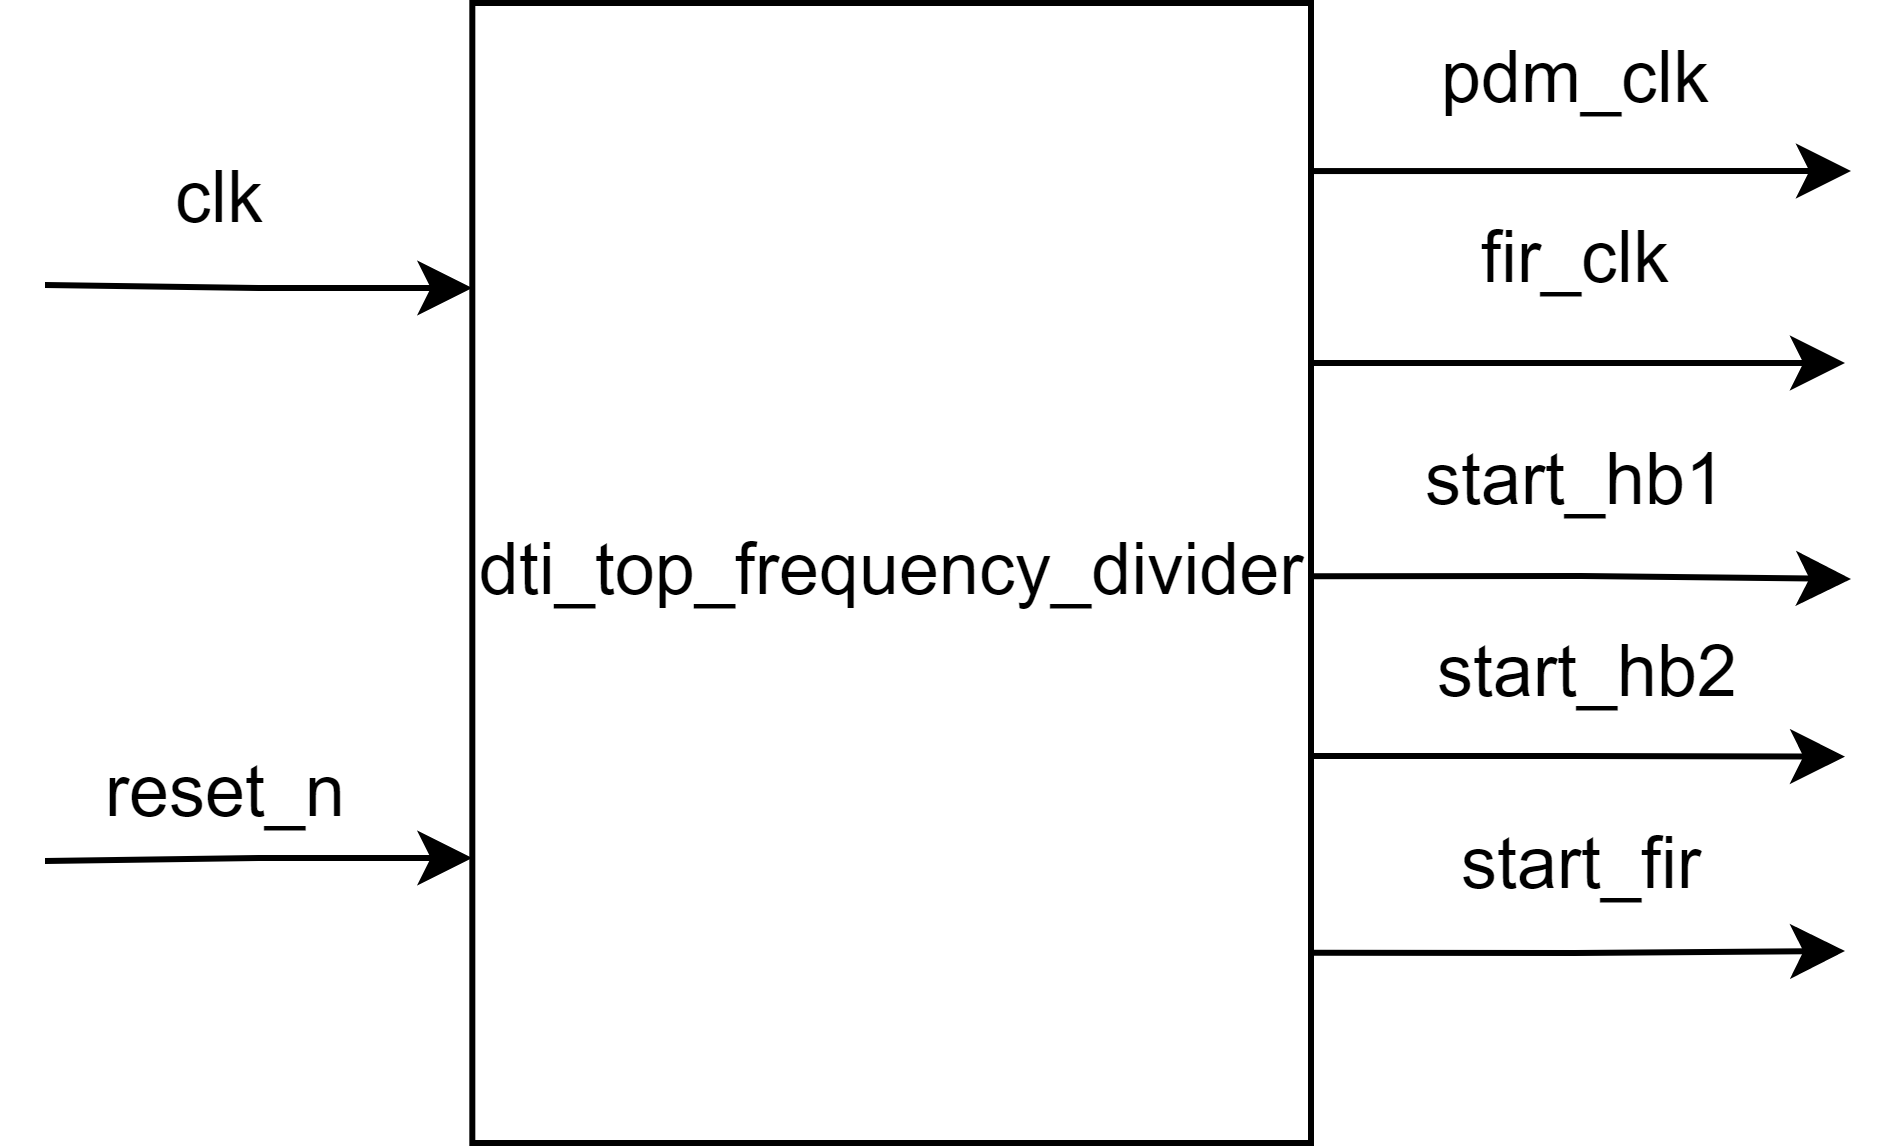
\includegraphics[width=8cm]{Images/Chuong4/frequency/top_frequency.png}
    \caption[Sơ đồ khối của dti\_top\_frequency\_divider]{\bfseries \fontsize{12pt}{0pt}\selectfont Sơ đồ khối của dti\_top\_frequency\_divider}
    \label{top_frequency}
\end{figure}
\begin{table}[H]
    \centering
    \caption[Mô tả chân vào ra của dti\_top\_frequency\_divider]{\bfseries\fontsize{12pt}{0pt}\selectfont Mô tả chân vào ra của dti\_top\_frequency\_divider}
    \begin{tabular}{|l|c|c|l|}
\hline
\multicolumn{1}{|c|}{\textbf{Tên chân}} &
  \textbf{Vào/ ra} &
  \textbf{Độ rộng bit} &
  \multicolumn{1}{c|}{\textbf{Mô tả chức năng}} \\ \hline
clk &
  vào &
  1 &
  Clock đồng bộ hoạt động của hệ thống \\ \hline
reset\_n &
  vào &
  1 &
  \begin{tabular}[c]{@{}l@{}}Chân reset không đồng bộ, tích cực mức\\ thấp\end{tabular} \\ \hline
start\_hb1 &
  ra &
  1 &
  \begin{tabular}[c]{@{}l@{}}Tín hiệu điều khiển cho biết liệu dữ liệu \\ có sẵn ở đầu vào của bộ lọc HB1\end{tabular} \\ \hline
start\_hb2 &
  ra &
  1 &
  \begin{tabular}[c]{@{}l@{}}Tín hiệu điều khiển cho biết liệu dữ liệu \\ có sẵn ở đầu vào của bộ lọc HB2\end{tabular} \\ \hline

\end{tabular}
    \label{top_frequency_signal}
\end{table}

\begin{table}[H]
    \centering
    % \caption[Mô tả chân vào ra của dti\_top\_frequency\_divider]{\bfseries\fontsize{12pt}{0pt}\selectfont Mô tả chân vào ra của dti\_top\_frequency\_divider}
    \begin{tabular}{|l|c|c|l|}
\hline
\multicolumn{1}{|c|}{\textbf{Tên chân}} &
  \textbf{Vào/ ra} &
  \textbf{Độ rộng bit} &
  \multicolumn{1}{c|}{\textbf{Mô tả chức năng}} \\ \hline
start\_fir &
  ra &
  1 &
  \begin{tabular}[c]{@{}l@{}}Tín hiệu điều khiển cho biết liệu dữ liệu \\ có sẵn ở đầu vào của bộ lọc FIR\end{tabular} \\ \hline
pdm\_clk &
  ra &
  1 &
  Clock lấy mẫu của PDM \\ \hline
pcm\_clk &
  ra &
  1 &
  Clock lấy mẫu của PCM \\ \hline
  \end{tabular}
  \end{table}

  Bảng \ref{top_frequency_signal} cho miêu tả chức năng của các chân vào ra của khối. Kiến trúc của dti\_top\_frequency\_divider gồm 4 bộ dti\_top\_frequency\_divider như hình \ref{top_frequency_arc}.

\begin{figure}[H]
    \centering
    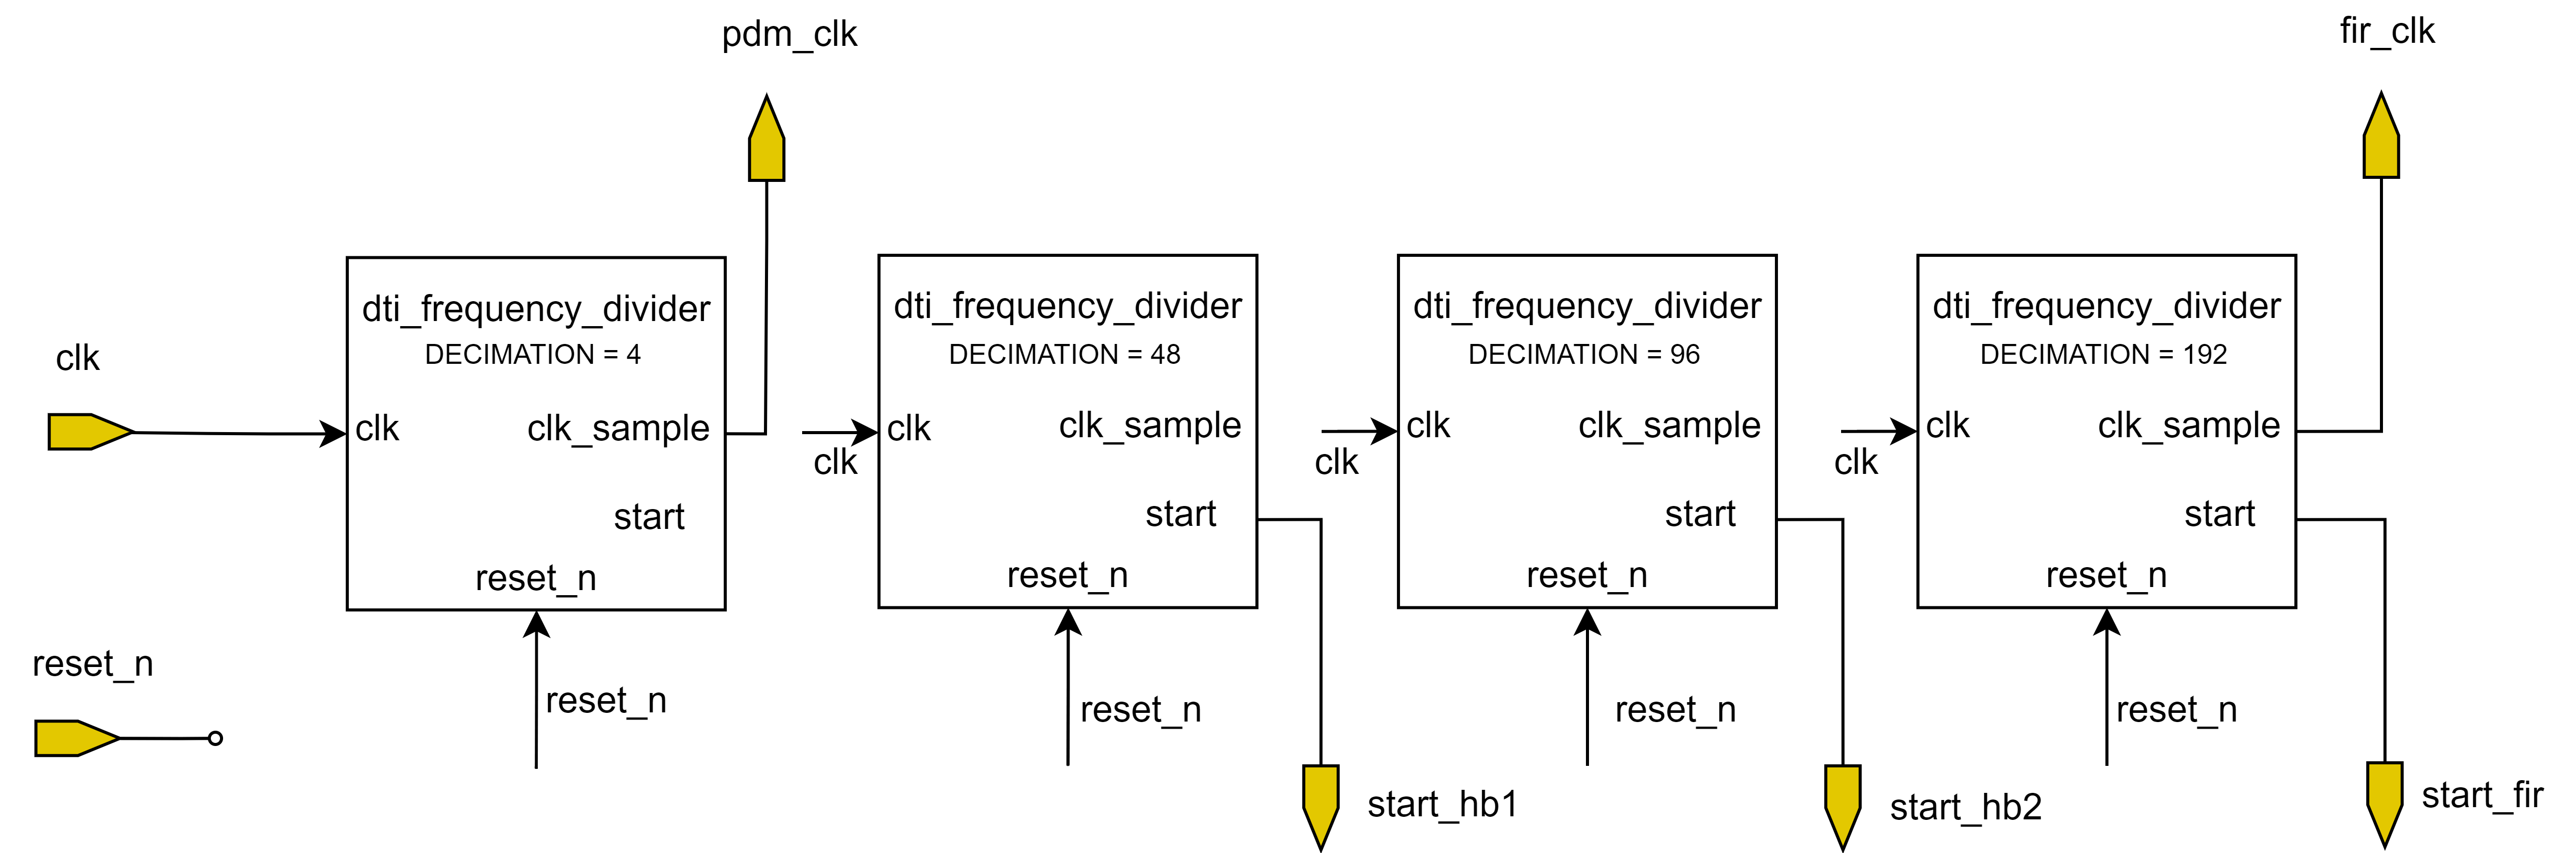
\includegraphics[width=15cm]{Images/Chuong4/frequency/top_frequency_arc.png}
    \caption[Kiến trúc của dti\_top\_frequency\_divider]{\bfseries \fontsize{12pt}{0pt}\selectfont Kiến trúc của dti\_top\_frequency\_divider}
    \label{top_frequency_arc}
\end{figure}

\paragraph{dti\_cic\_decimator}
 Như đã trình bày ở mục \ref{cic_filter_ref}, với thiết kế bộ lọc CIC 4 tầng và hệ số Decimation 12x thì chúng ta cần đến 4 bộ cộng và 4 bộ trừ. Chúng ta có thể tăng tần số xử lý lên 4 lần, lúc này chỉ cần sử dụng 1 bộ cộng và 1 bộ trừ, điều này làm giảm tài nguyên phần cứng một cách đáng kể.

Hình \ref{cic_top} mô tả sơ đồ khối của khối dti\_cic\_decimator.
\begin{figure}[H]
    \centering
    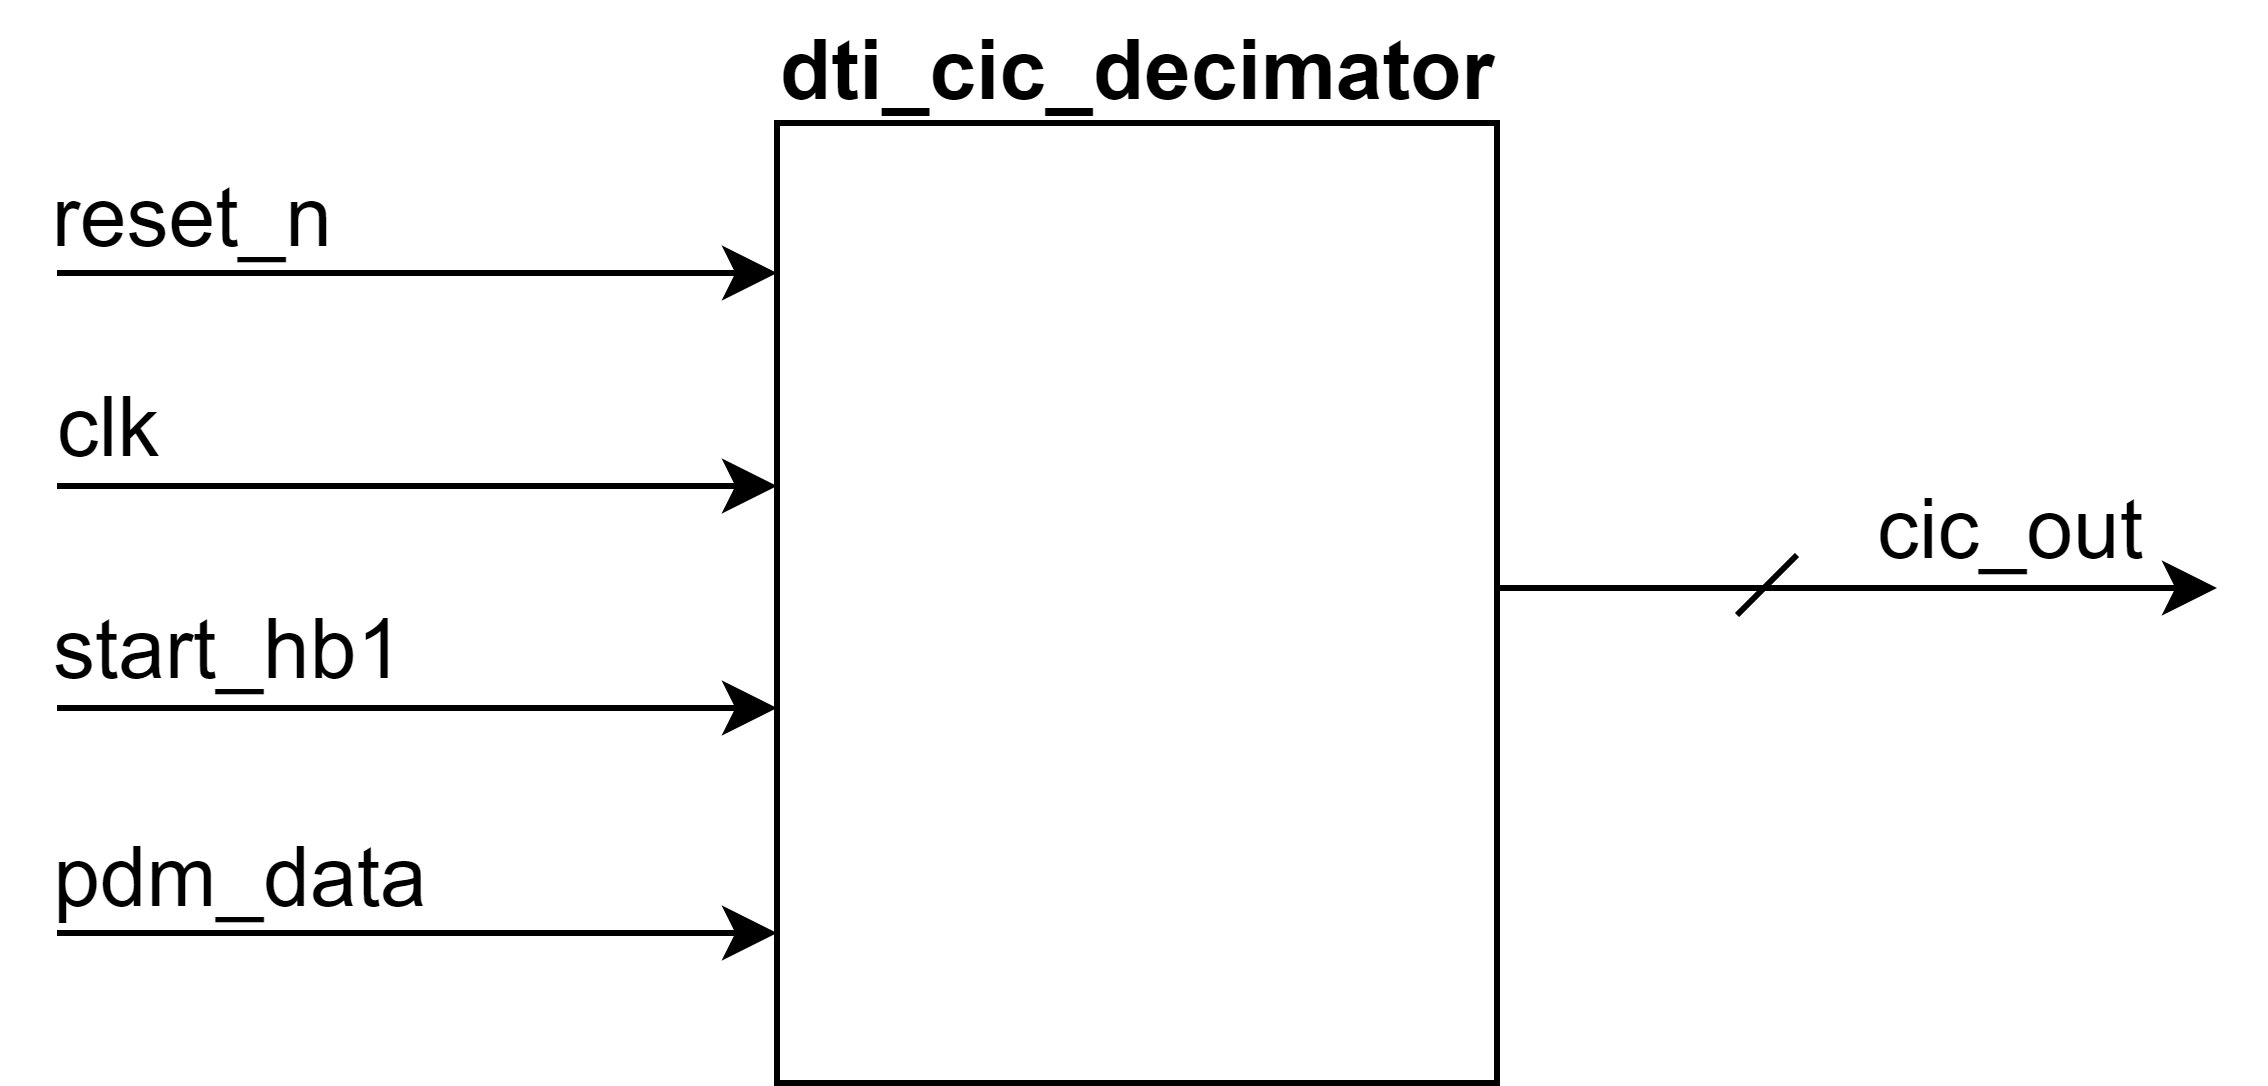
\includegraphics[width=10cm]{Images/Chuong4/cic/cic_top.png}
    \caption[Sơ đồ khối của dti\_cic\_decimator]{\bfseries \fontsize{12pt}{0pt}\selectfont Sơ đồ khối của dti\_cic\_decimator}
    \label{cic_top}
\end{figure}

Việc tính toán độ rông bit cho các thanh ghi trễ được tính toán theo công thức \ref{bitcic}. Với số tầng là 4 và hệ số Decimation 12x ta có độ rộng bit như sau:
\begin{equation}
    n_r = 1 + [4 \times log_2(2 \times 12)] = 16 (bits)
\end{equation}
\begin{table}[H]
    \centering
    \caption[Mô tả chân vào ra của dti\_cic\_decimator]{\bfseries\fontsize{12pt}{0pt}\selectfont Mô tả chân vào ra của dti\_cic\_decimator}
    \begin{tabular}{|l|c|c|l|}
\hline
\multicolumn{1}{|c|}{\textbf{Tên chân}} &
  \textbf{Vào/ ra} &
  \textbf{Độ rộng bit} &
  \multicolumn{1}{c|}{\textbf{Mô tả chức năng}} \\ \hline
clk       & vào & 1 & Clock đồng bộ hoạt động của hệ thống \\ \hline
reset\_n &
  vào &
  1 &
  \begin{tabular}[c]{@{}l@{}}Chân reset không đồng bộ, tích cực mức\\ thấp\end{tabular} \\ \hline
start\_hb1 &
  vào &
  1 &
  \begin{tabular}[c]{@{}l@{}}Báo hiệu rằng dữ liệu đầu ra CIC thay đổi\\ (bộ lọc HB1 nhận dữ liệu)\end{tabular} \\ \hline
pdm\_data & vào & 1 & Dữ liệu PDM đầu vào                  \\ \hline
pcm\_data &
  ra &
  16 &
  \begin{tabular}[c]{@{}l@{}}Đầu ra của bộ lọc CIC, tiếp tục đưa vào \\ bộ lọc HB1\end{tabular} \\ \hline
\end{tabular}
    \label{cic_top_t}
\end{table}

Bảng \ref{cic_top_t} liệt kê các cổng vào ra của khối dti\_cic\_decimator. Khi chỉ sử dụng một bộ công và 1 bộ cộng, chúng ta phải phân công theo từng thời gian tính toán các phép tính 1 cách hợp lý, hình \ref{cic_top_arc} mô tả kiến trúc đáp ứng được điều kiện trên.

\begin{figure}[H]
    \centering
    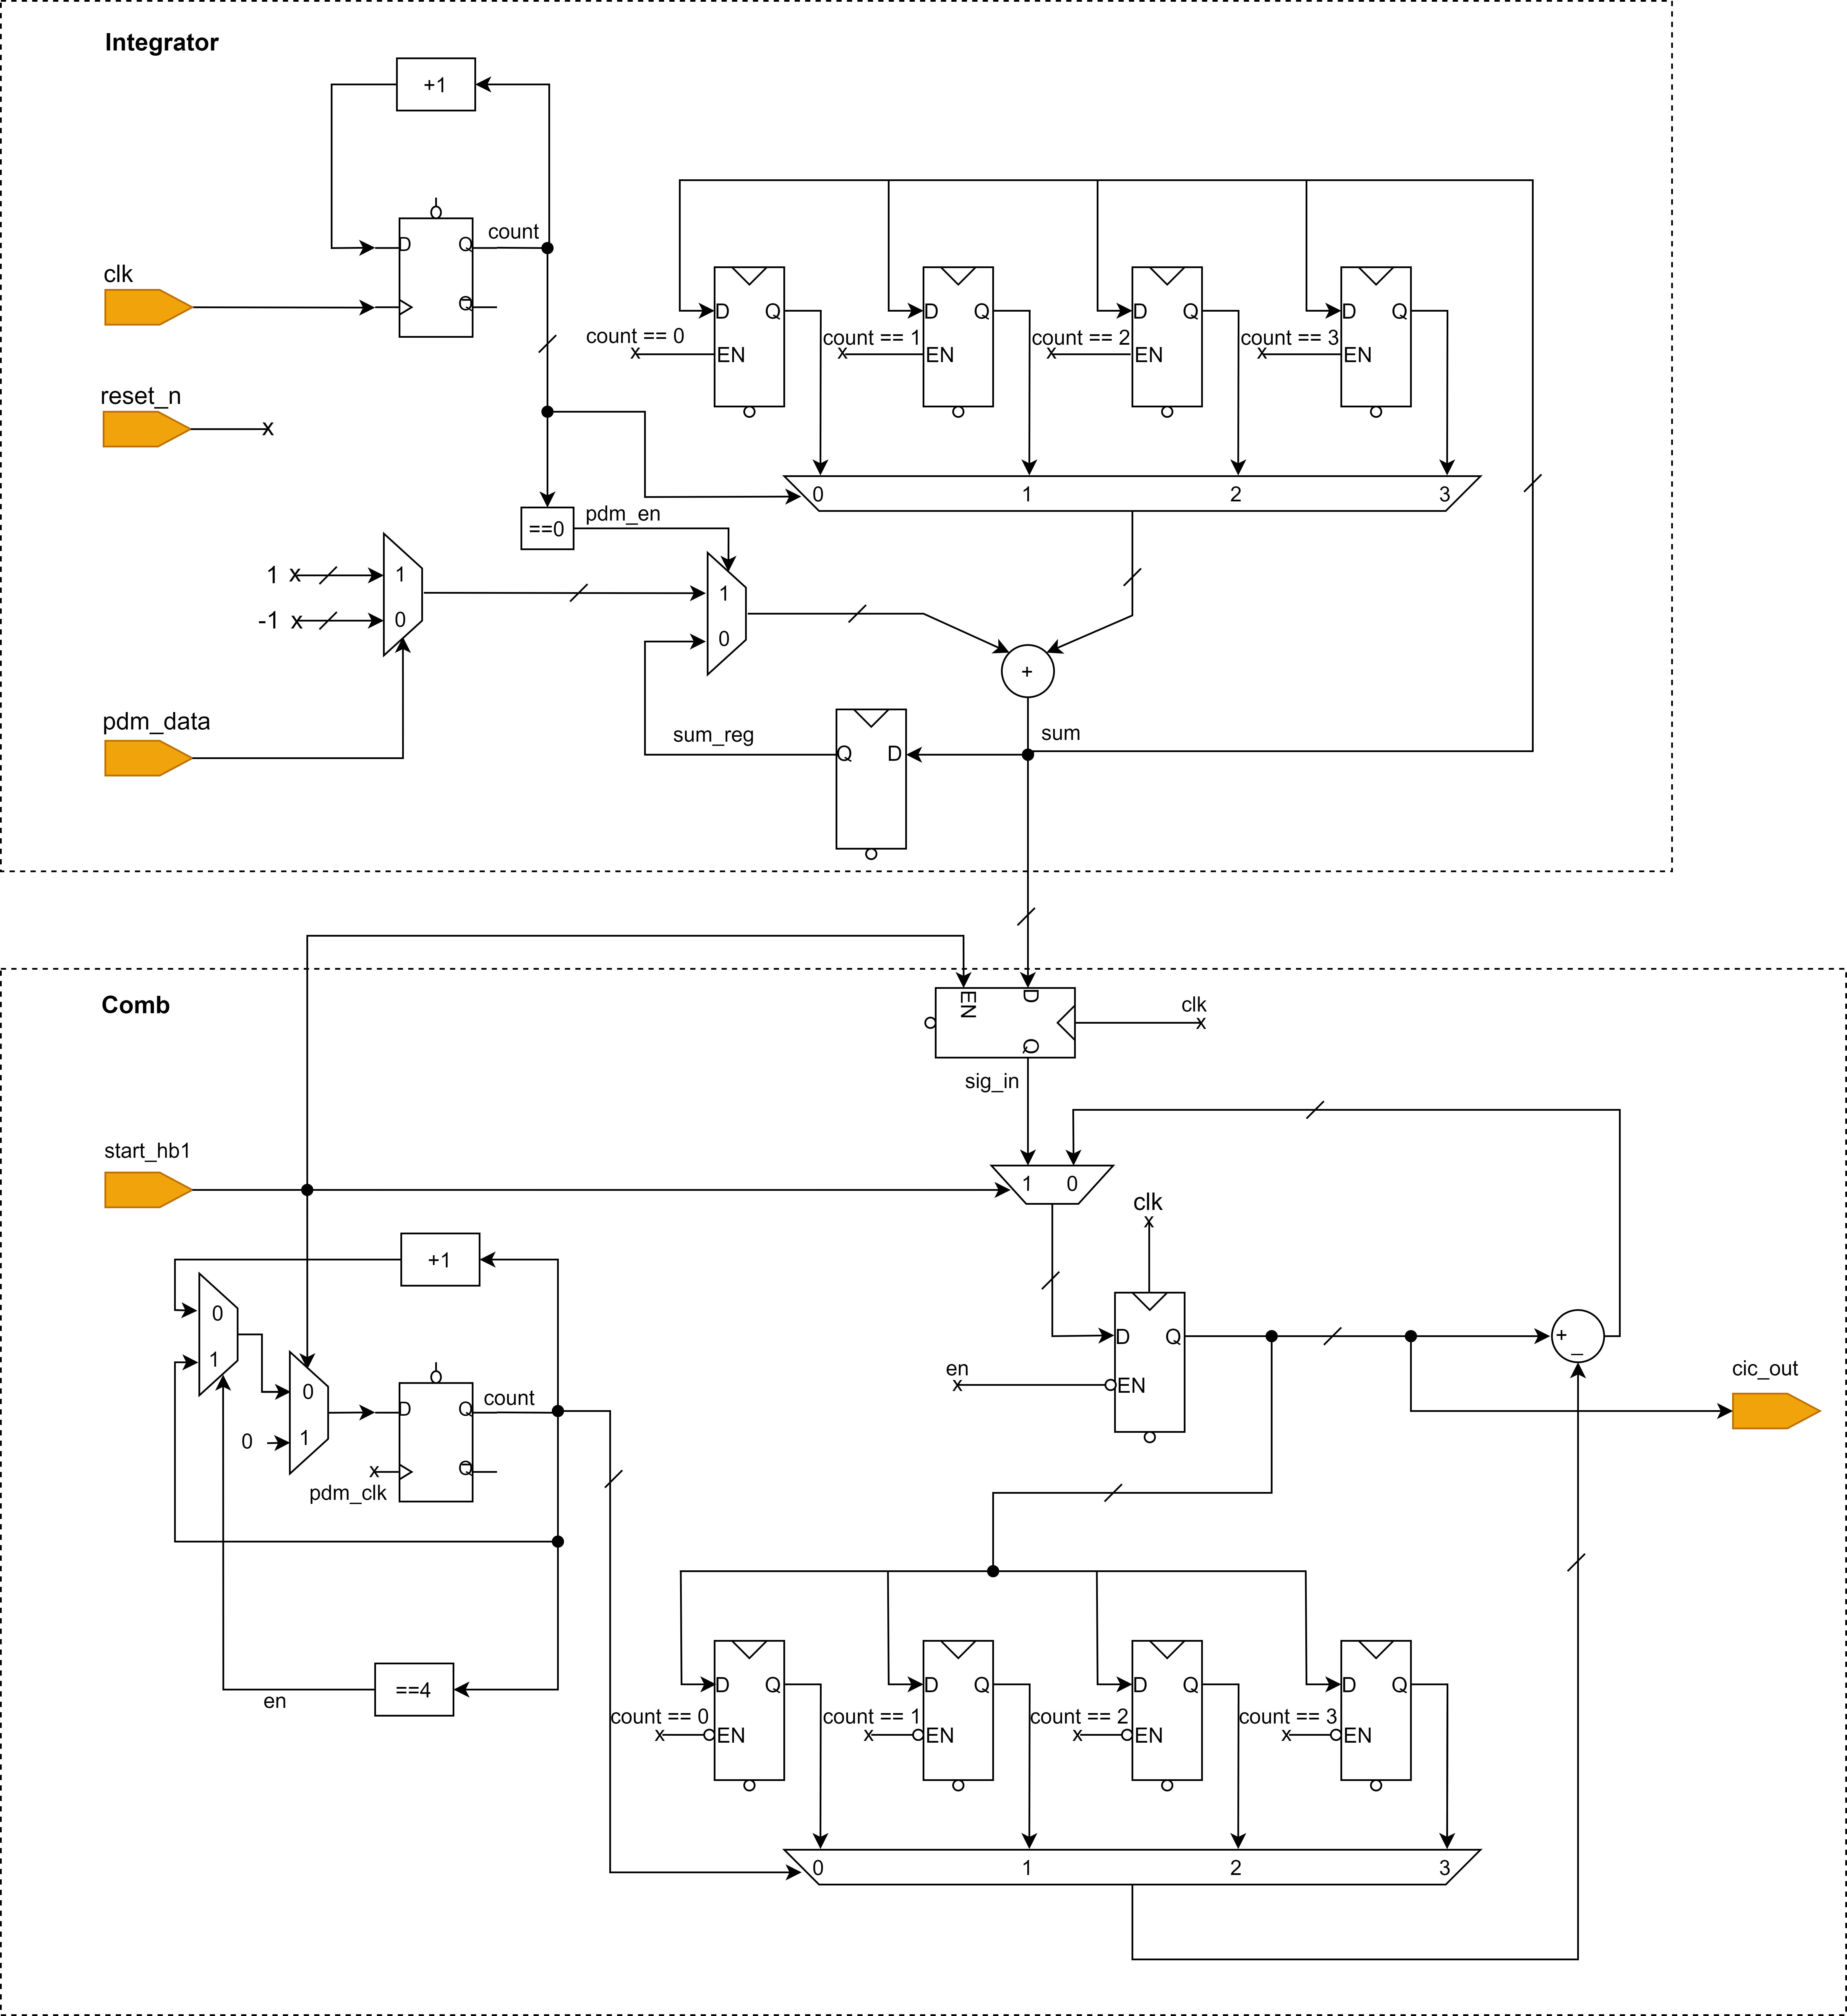
\includegraphics[width=16cm]{Images/Chuong4/cic/cic_top_arc.png}
    \caption[Kiến trúc của dti\_cic\_decimator]{\bfseries \fontsize{12pt}{0pt}\selectfont Kiến trúc của dti\_cic\_decimator}
    \label{cic_top_arc}
\end{figure}
 \paragraph{dti\_hb\_fir\_filter}
Tương tự bộ lọc CIC, 3 bộ lọc tiếp theo cũng phải sử dụng số bộ nhân và bộ cộng nhất định:
\begin{itemize}
    \item Half Band (1): có 11 taps, trong đó 4 taps có hệ số bằng 0 coi như không sử dụng bộ nhân ở đây. Đồng nghĩa với việc chúng ta cần phải có 7 bộ nhân và 10 bộ cộng cho bộ HB1.
     \item Half Band (2): có 19 taps. Tương tự cách tính của HB1, HB2 cần 11 bộ nhân và 18 bộ cộng.
     \item FIR: có 51 taps nên sẽ sửa dụng 51 bộ nhân và 50 bộ cộng.
\end{itemize} 

Không những thế bộ nhân là bộ có kích thước khá lớn, việc sử dụng số lượng nhiều sẽ gây tiêu tốn tài nguyên. Ý tưởng của kiến trúc này là chỉ sử dụng 1 bộ nhân duy nhất cho 3 bộ lọc và mỗi bộ lọc sử dụng 2 bộ cộng.

\begin{figure}[H]
    \centering
    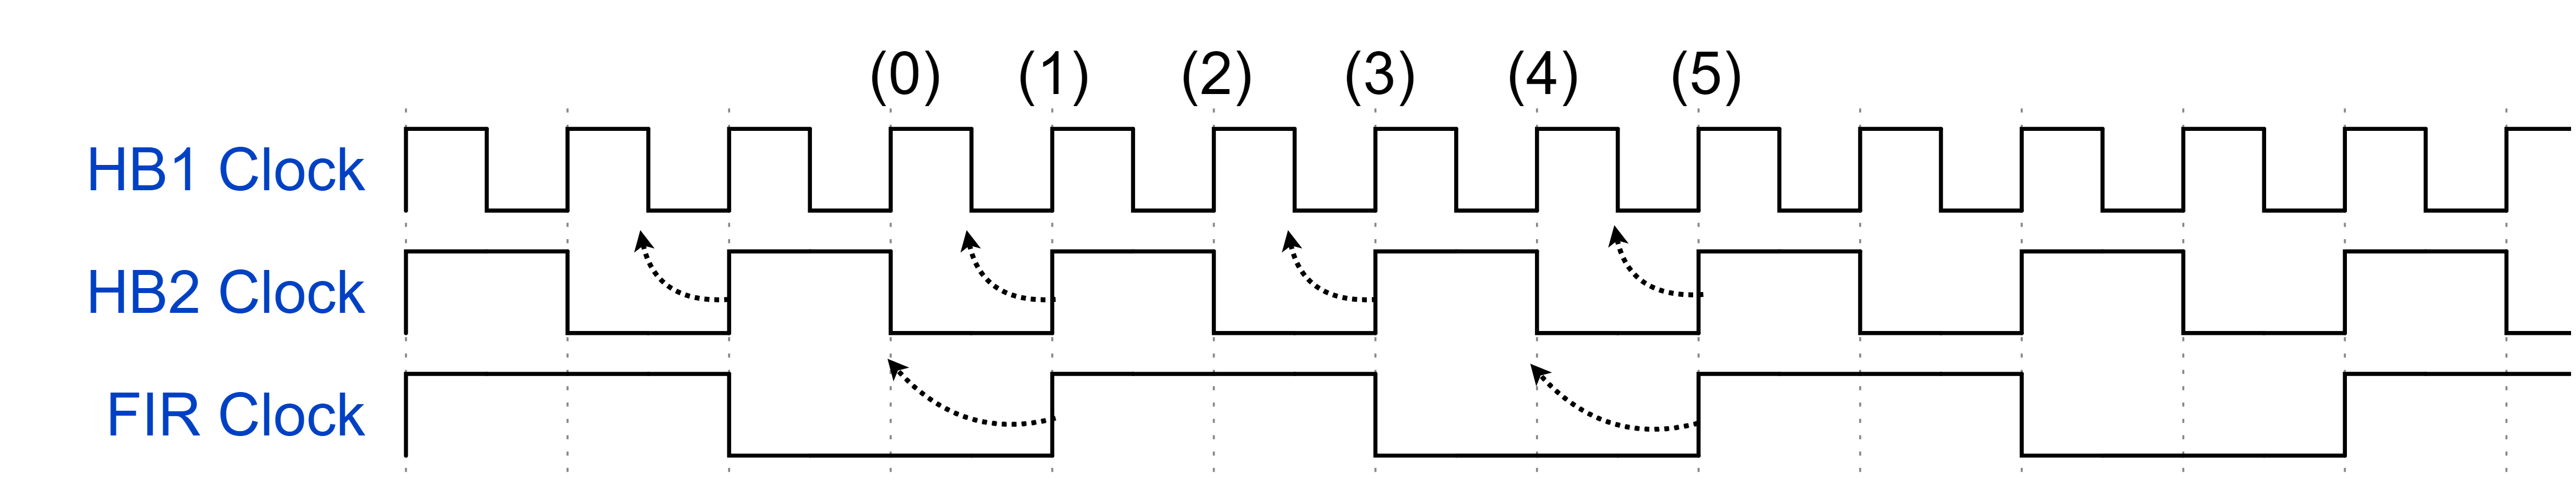
\includegraphics[width=16cm]{Images/Chuong4/hb_fir/timing.png}
    \caption[Biểu đồ thời gian của 3 clock của 3 bộ lọc]{\bfseries \fontsize{12pt}{0pt}\selectfont Biểu đồ thời gian của 3 clock của 3 bộ lọc}
    \label{3clock}
\end{figure}

Quan sát biểu đồ thời gian của 3 clock (hình \ref{3clock}), ta có nhận xét sau: không phải tất cả ở sườn dương nào thì các bộ lọc đều phải tính toán. Việc tính toán hay không là do bộ lọc sau lấy giá trị ở thời điểm nào để tính toán. Ví dụ với bộ lọc HB2, nó chỉ lấy giá trị đầu ra của HB1 sau thời điểm (0), (2), (4) điều này đồng nghĩa với việc ở đây HB1 phải thực hiện các phép toán ở (0), (2), (4) để xuất tín hiệu cho đầu vào HB2, ở các điểm còn lại HB1 chỉ cần dịch giá trị đầu vào vào và không làm thêm gì. Điều đó tương tự với bộ lọc FIR, nó chỉ lấy đầu vào của HB2  sau thời điểm (3) để tính toán.

Dựa vào cách hoạt động trên, ta có thể tiến hành để mỗi bộ lọc sử dụng bộ nhân ở 1 thời điểm nhất định. Với ví dụ trên thứ tự sử dụng bộ nhân sẽ như sau: (0) - HB1, (1) - FIR, (2) - HB1, (3) - HB2 và lặp lại. Việc phân luồng sẽ có do bộ \textbf{dti\_filter\_controller} điều khiển.

Do bộ FIR sẽ có 52 taps, đồng nghĩa với việc trong 1 chu kỳ của HB1 phải thực hiện xong 26 lần nhân (vì hệ số đối xứng). Ta xét tần số hoạt động của HB1 là 192 kHz thì tần hoạt động của bộ nhân phải là $192 \times 26 = 4492 kHz$. Với tần số của hệ thống sử dụng (dti\_cic\_decimatior clock) là 9216 khz đã hoàn toàn đáp ứng được.

\begin{figure}[H]
    \centering
    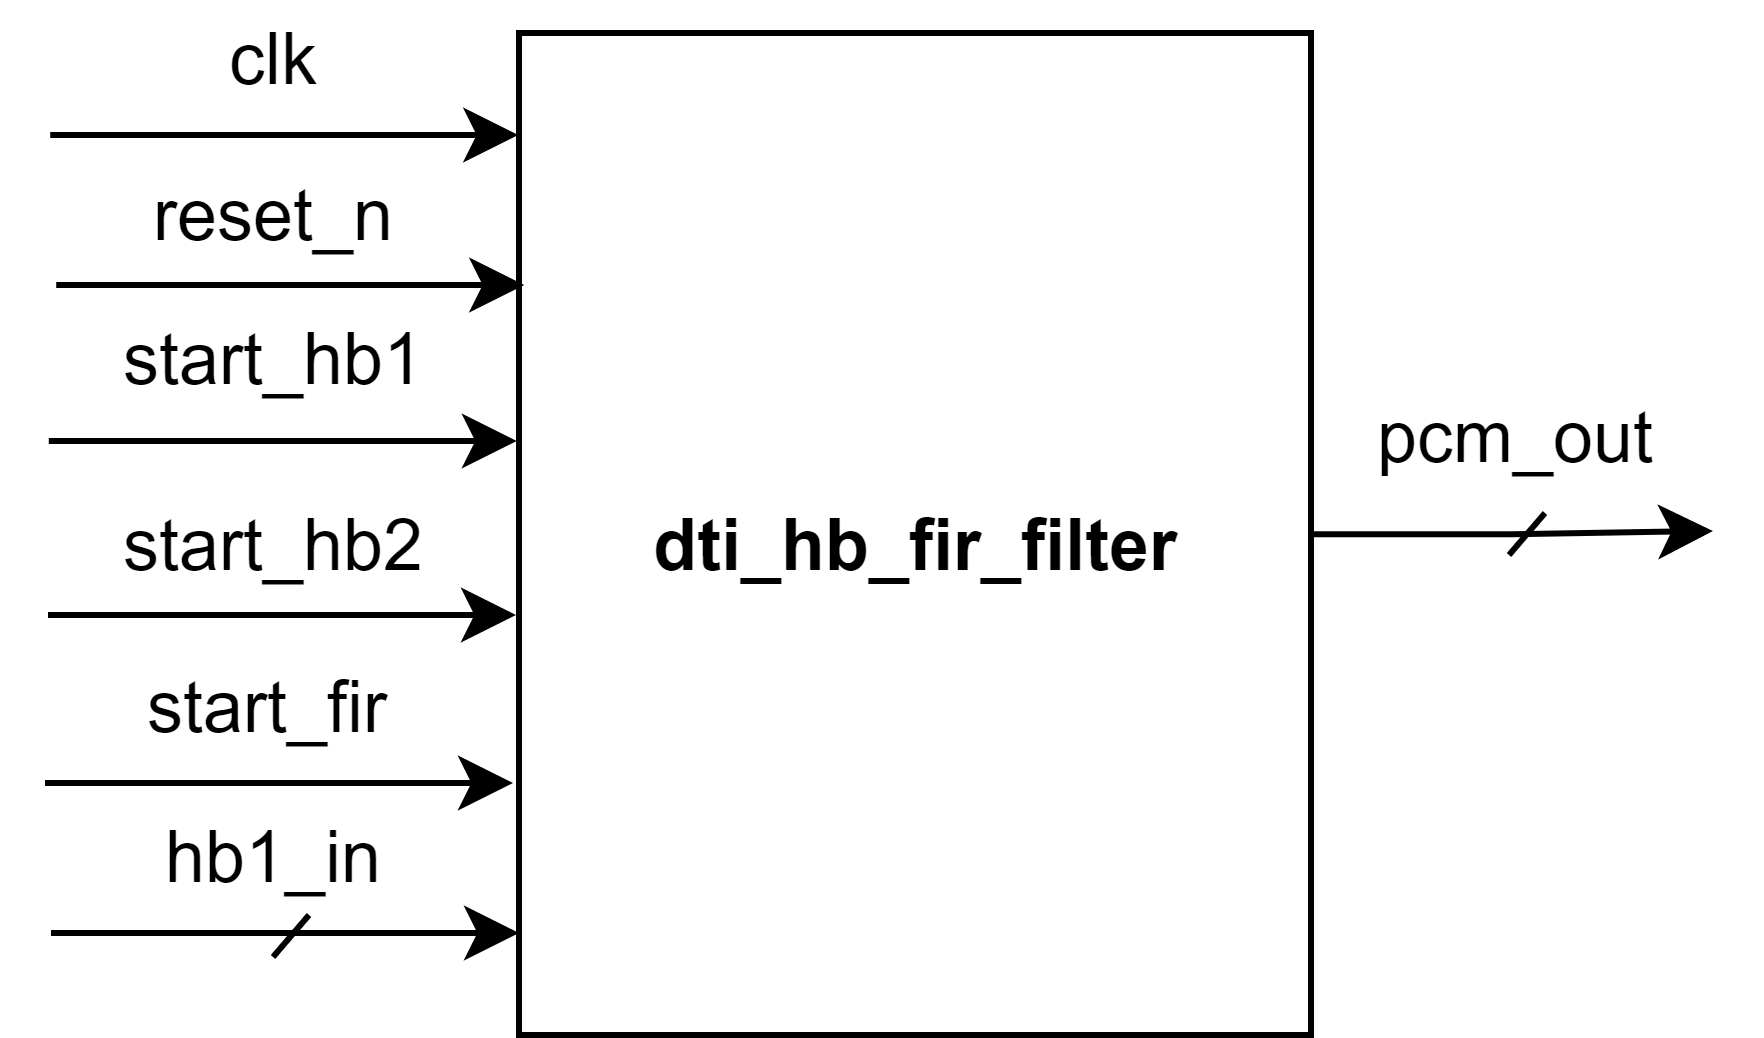
\includegraphics[width=8cm]{Images/Chuong4/hb_fir/hb_fir_top.png}
    \caption[Sơ đồ khối của dti\_cic\_decimator]{\bfseries \fontsize{12pt}{0pt}\selectfont Sơ đồ khối của dti\_hb\_fir\_filter}
    \label{hb_fir_top}
\end{figure}
Hình \ref{hb_fir_top} mô tả sơ đồ khối của khối dti\_hb\_fir\_filter.

\newpage